\clearpage

\appendix

\renewcommand{\thesection}{\Alph{section}}
\renewcommand{\thefigure}{\Alph{section}.\arabic{figure}}
\setcounter{figure}{0}

\section{Debugging \LaTeX\ integration with LANS}

are working under Microsoft Windows, you can fix this problem by compiling the \ttt{tex} file using the native \LaTeX\ environment (e.g., open the \ttt{tex} file in the default editor of your \LaTeX\ distribution and then compile it into a \ttt{pdf} output from there). When doing so, the missing \LaTeX\ packages should automatically be installed and the \ttt{tex} file should compile into a~correct \ttt{pdf} output. Once this is done, the automatic \LaTeX\ compilation from within Matlab will also work.

If you are using Linux or MacOS, you need to do a~little bit of internet searching to figure out how to ensure that all the required \LaTeX\ packages are installed.


%%%

\section[Appendix]{Hierarchical data structure implemented in LANS}

\begin{figure}[!hb]
\centering
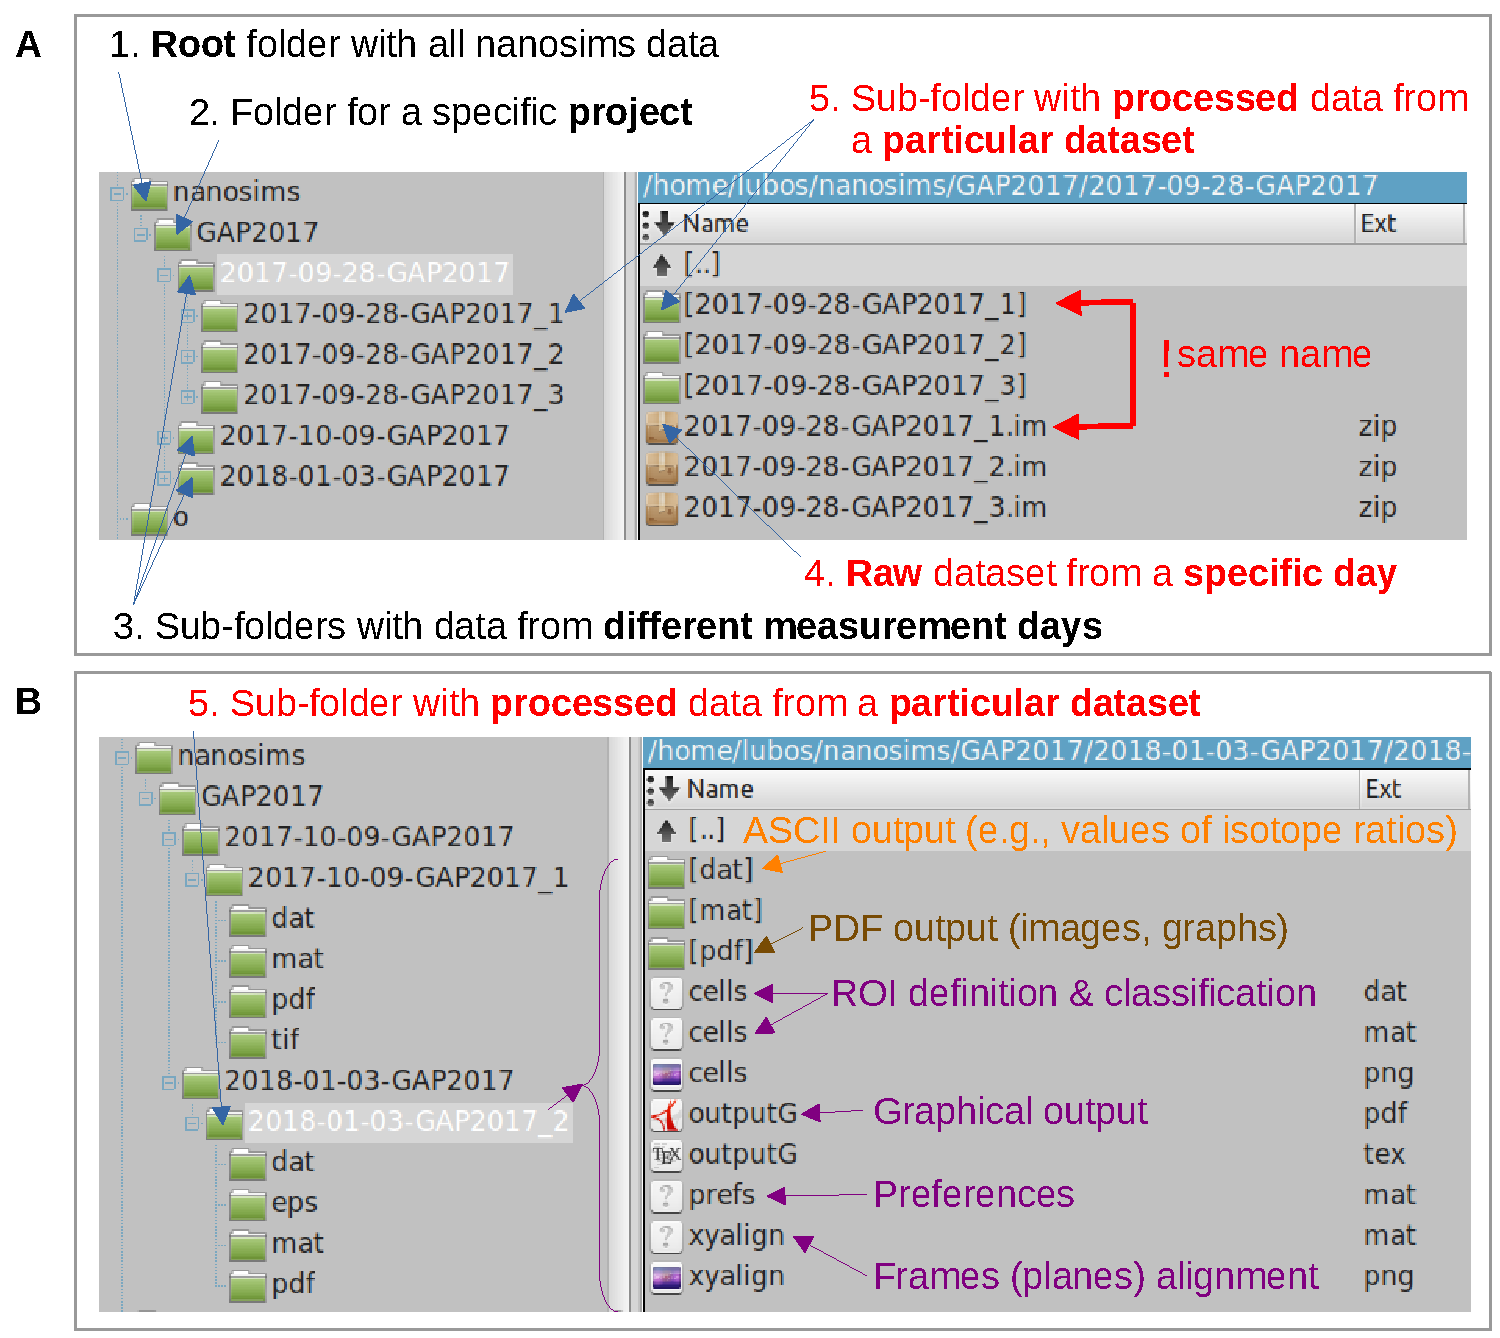
\includegraphics[scale=0.41]{figs2/folders_organizationAB}\\
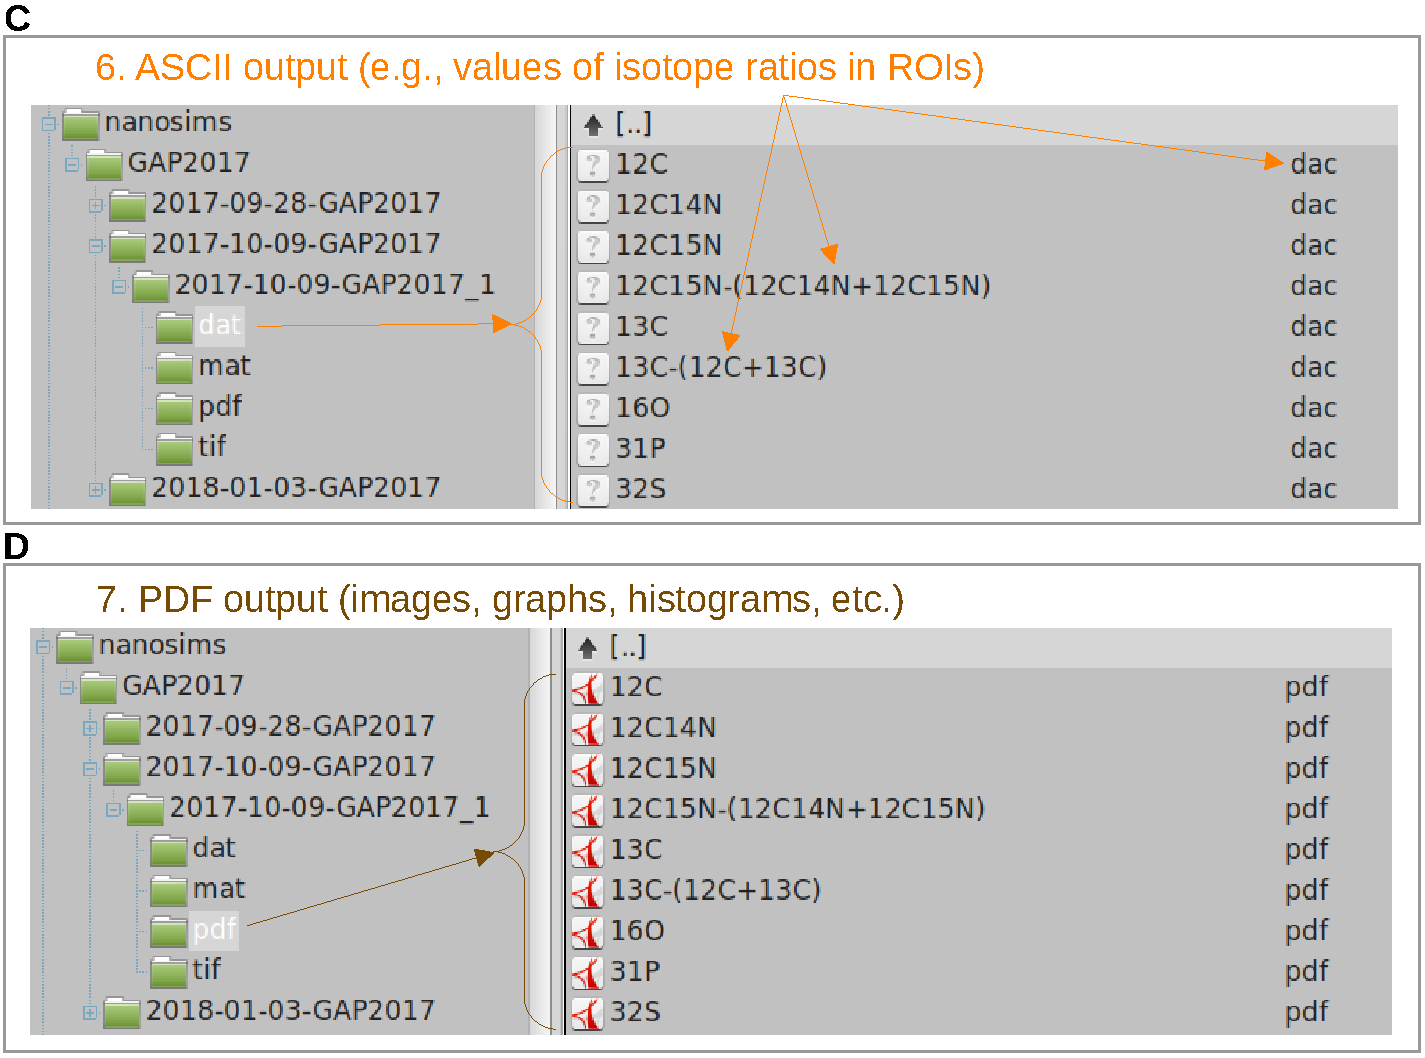
\includegraphics[scale=0.41]{figs2/folders_organizationCD}
\caption{\label{fig2:data_organization}%
	Example of a hierarchical organization of the raw and processed nanoSIMS data implemented in Look@NanoSIMS. %
  \textbf{(A)} The root folder (\ttt{nanosims}) contains a~project-specific sub-folder (e.g., \ttt{GAP2017}), which contains sub-folders with data measured on different days (e.g., \ttt{2017-09-28-GAP2017}, \ttt{2017-10-09-GAP2017}). %
  The `day folder' contains \emph{multiple raw datasets} measured on that particular day (\ttt{im} or \ttt{im.zip} files). %
  When a particular raw dataset is processed and analyzed, the data is stored in a `dataset folder' with the \emph{same name} as the dataset (see red ``!''). %
  \textbf{(B)} The `dataset folder' contains files defining the processing steps, including alignment information (\ttt{xyalign}), definition and classification of regions of interest (\ttt{cells.mat} and \ttt{cells.dat}, respectively), preferences (\ttt{prefs.mat}), and a comprehensive summary of results exported in a PDF file (\ttt{OutputG.pdf}). %
  The `dataset folder' also contains sub-folders with output generated by LANS in different formats. %
    \textbf{(C)} The ROI-specific ion counts and ion count ratios (\ttt{dac} files) are stored in the \ttt{dat} folder. %
    \textbf{(D)} The images, graphs, histograms, etc., are stored in the \ttt{pdf} folder.}%
\end{figure}
